\documentclass[tikz]{standalone}
\usepackage{tikz}

\begin{document}    
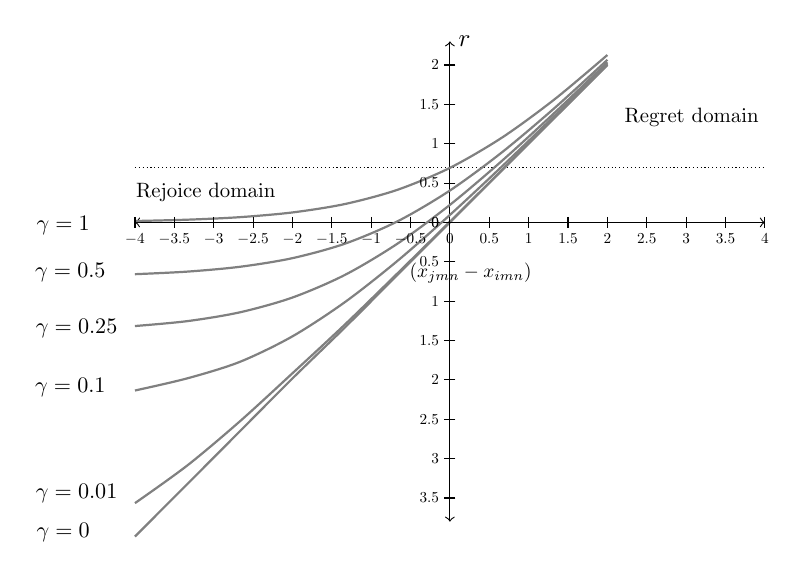
\begin{tikzpicture}
 \usetikzlibrary{positioning}
 \node (center) {};
 
 
 %Coordinates
 \coordinate (RRMcoordinate) at (0.5,1);

 
 %Name
 %\node (GRRM) [scale=0.7,  above right =1cm and -5.34cm   of center] { $R^{GRRM}_{i\leftrightarrow jmn}=\ln\left\{\gamma + \exp\left[\beta_{m}\cdot\left(x_{jmn} - x_{imn}\right)\right]\right\}$};
  \node (regret) [scale=0.75,above right=1cm and 2cm of center,black ] {Regret domain};
\node (rejoice) [scale=0.75,above left=0.05cm and 2cm of center,black ] {Rejoice domain};

\node (GRRM1) [scale=0.8,  below left =-0.3cm and 4.35cm of center] { $\gamma=1$};
\node (GRRM05) [scale=0.8,  below left =0.3cm and 4.15cm of center] { $\gamma=0.5$};
\node (GRRM05) [scale=0.8,  below left =1cm and 4cm of center] { $\gamma=0.25$};
\node (GRRM05) [scale=0.8,  below left =1.75cm and 4.15cm of center] { $\gamma=0.1$};
\node (GRRM05) [scale=0.8,  below left =3.1cm and 4cm of center] { $\gamma=0.01$};
\node (GRRM05) [scale=0.8,  below left =3.6cm and 4.35cm of center] { $\gamma=0$};


 
 %Axis
   \draw[<->] (-4, 0) -- (4, 0) node[scale=0.7,below left= 0.3cm and -1.25cm of center] {$(x_{jmn} - x_{imn})$};
  \draw[<->] (0, -3.8) -- (0, 2.3) node[right,scale=0.9] {$r$};
  
 %Functions
   \draw[scale=1, domain=-4:4, densely dotted ,variable=\x, black] plot  ({\x}, {ln(2)});

  
  \draw[scale=1, samples=10 ,domain=-4:2, smooth ,variable=\x, gray,thick] plot  ({\x}, {ln(1+exp(\x))});
  \draw[scale=1, samples=10 ,domain=-4:2, smooth ,variable=\x, gray,thick] plot  ({\x}, {ln(0.5+exp(\x))});
  \draw[scale=1, samples=10 ,domain=-4:2, smooth ,variable=\x, gray,thick] plot  ({\x}, {ln(0.25+exp(\x))});
  \draw[scale=1, samples=10 ,domain=-4:2, smooth ,variable=\x, gray,thick] plot  ({\x}, {ln(0.1+exp(\x))});
  \draw[scale=1, samples=10 ,domain=-4:2, smooth ,variable=\x, gray,thick] plot  ({\x}, {ln(0.01+exp(\x))});
  \draw[scale=1, samples=10 ,domain=-4:2, smooth ,variable=\x, gray,thick] plot  ({\x}, {ln(0.0+exp(\x))});


 \foreach \x/\xtext in {0,0.5,1,1.5,2,2.5,3,3.5,4}
\draw[shift={(\x,0)}] (0pt,2pt) -- (0pt,-2pt) node[scale=0.55,below] {$\xtext$};

 \foreach \x/\xtext in {0.5,1,1.5,2,2.5,3,3.5,4}
\draw[shift={(-\x,0)}] (0pt,2pt) -- (0pt,-2pt) node[scale=0.55,below] {$-\xtext$};

  \foreach \y/\ytext in {0,0.5,1,1.5,2}
  \draw[shift={(0,\y)}] (2pt,0pt) -- (-2pt,0pt) node[scale=0.55,left] {$\ytext$};
  
  \foreach \y/\ytext in {0,0.5,1,1.5,2,2.5,3,3.5}
\draw[shift={(0,-\y)}] (2pt,0pt) -- (-2pt,0pt) node[scale=0.55,left] {$\ytext$};

  %Labels of functions

  
\end{tikzpicture}
\end{document}


